\addcontentsline{toc}{chapter}{Anexo}
\chapter{Art�culos posteriores a la Comisi�n de Doctorado de Abril de 2009.}
\newpage

Art�culos manuscritos enviados o pendientes de publicaci�n posteriores a la Comisi�n de Doctorado de la UAB en Abril de 2009:

\begin{enumerate}[a)]
\item \textsc{Polyanionic Carbosilane And Carbosiloxane Metallodendrimers Based On Cobaltabisdicarbollide Derivatives.}
 Emilio Jos� Ju�rez-P�rez, Clara Vi�as, Francesc Teixidor, Rosario N��ez.
 \emph{Organometallics} \textbf{2009}, \textit{submitted}.

\item \textsc{Polyanionic Aryl-Ether Metallodendrimers Based On Cobaltabisdicarbollide Derivatives. Photoluminescent Properties.}
 Emilio Jos� Ju�rez-P�rez, Clara Vi�as, Francesc Teixidor, Rosa Santillan, Norberto Farf�n, Arturo Abreu, Rebeca
Y�pez, Rosario N��ez. \textit{In preparation}.

\item \textsc{Decorating Poly(Alkyl Aryl-Ether) Dendrimers With Metallacarboranes.}
Rosario N��ez, Emilio Jos� Ju�rez-P�rez, Francesc Teixidor, Rosa Santillan, Norberto Farf�n, Arturo Abreu, Rebeca
Y�pez, Clara Vi�as. \textit{In preparation}.

\item \textsc{Anchoring Phosphorous-containing Cobaltabisdicarbollide Derivatives on Titania Particles.}
 Emilio Jos� Ju�rez-P�rez, Hubert Mutin, Michel Granier, Francesc Teixidor, Rosario N��ez. \textit{In preparation}.

\item \textsc{Approaches For Anchoring Cobaltabisdicarbollide Anions Onto Oxidized Silicon Wafers.}
 Emilio Jos� Ju�rez-P�rez, Michel Granier, Hubert Mutin, Clara Vi�as, Rosario N��ez. \textit{In preparation}.

\item \textsc{Thumb Rules to Establish the Rotamer Configuration in Metallacarborane Sandwiches. The relevance of the \ce{C_c-H}$\cdot \cdot \cdot$\ce{H-B} Self Interactions.}
 Emilio J. Ju�rez-P�rez, Rosario N��ez, Clara Vi�as, Reijo Sillanp��, Francesc Teixidor.
 \emph{Inorg. Chem.} \textbf{2009}, \textit{submitted}.


\end{enumerate}

\clearpage
\subsubsection{a) Polyanionic Carbosilane And Carbosiloxane Metallodendrimers Based On Cobaltabisdicarbollide Derivatives.}
\cleardoublepage
\newpage
\clearpage
\tb{0.9}{0.5}{0.55}{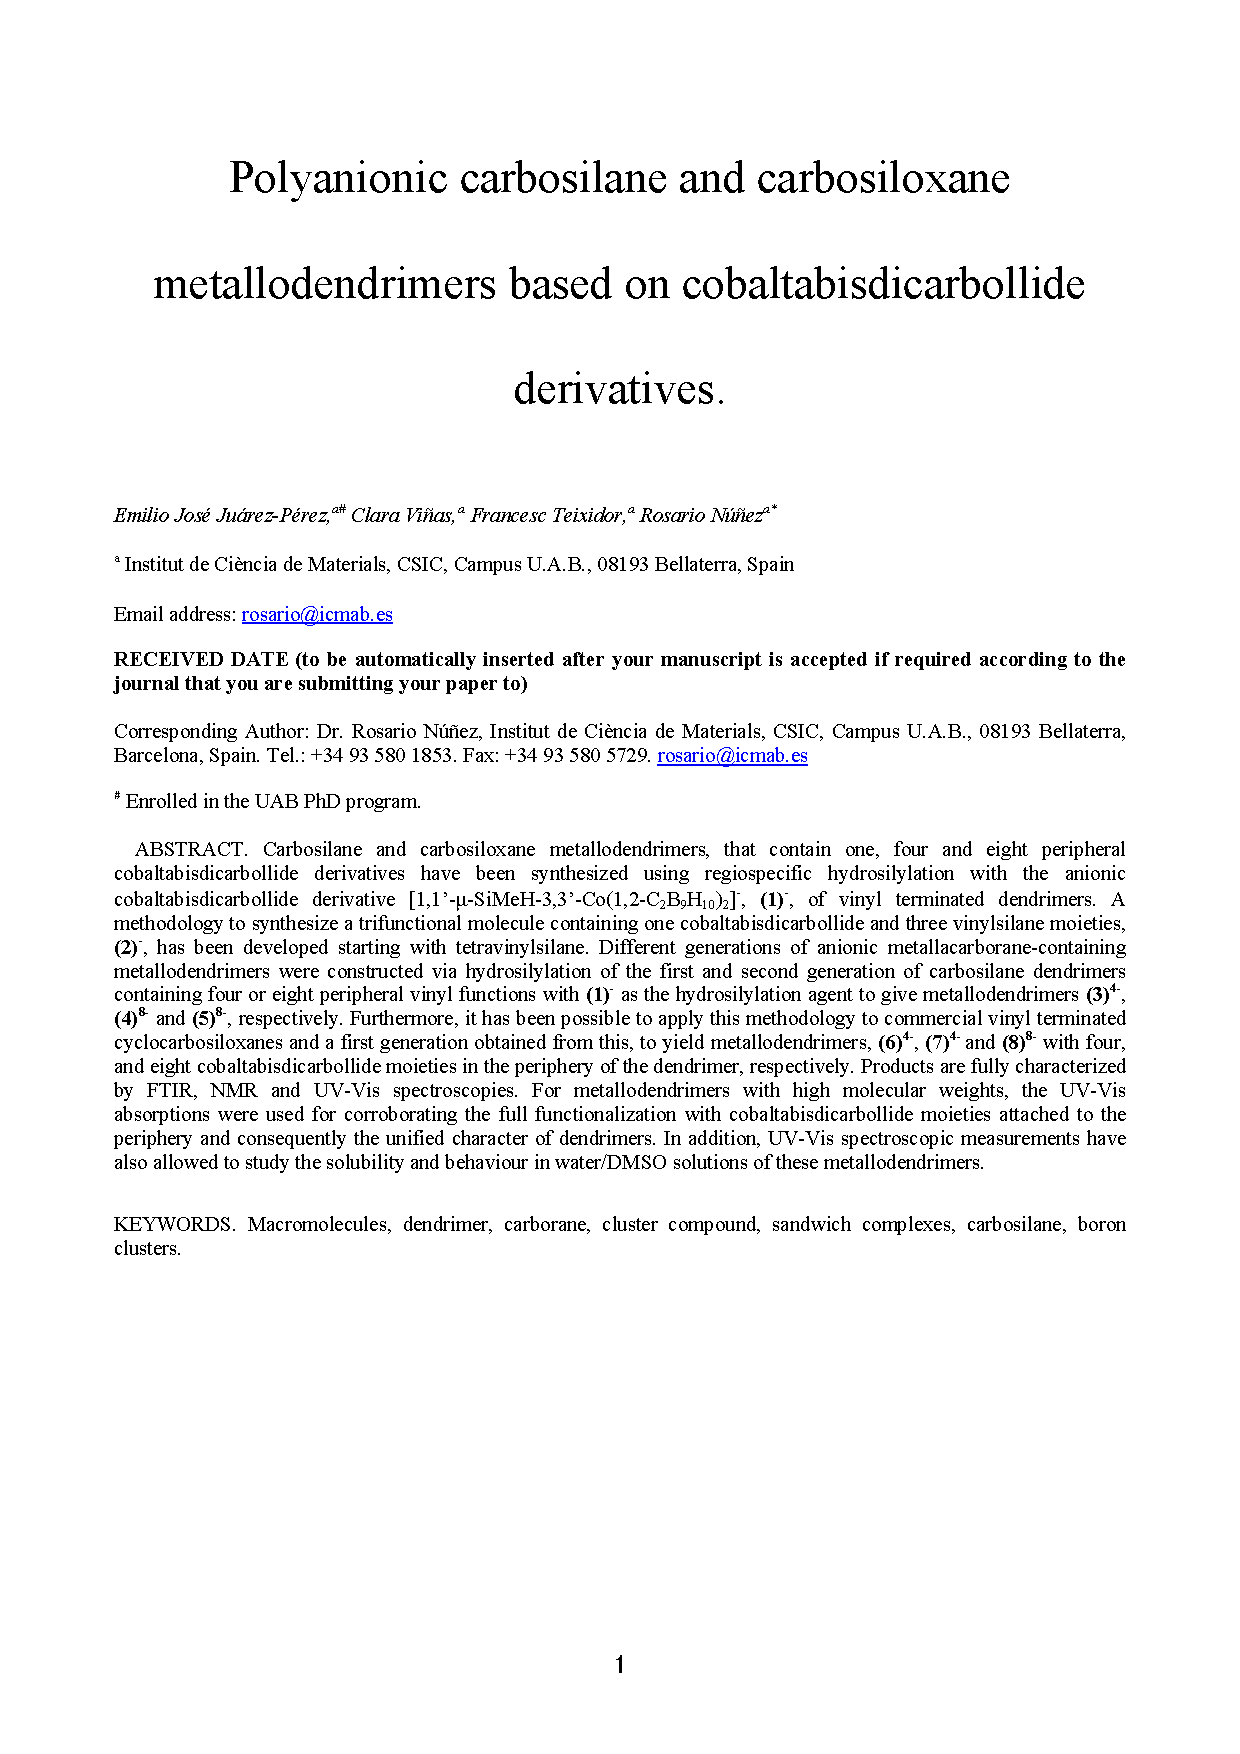
\includegraphics [width =1 \textwidth ]{figuras/articulos/1-art4.pdf}} \null \newpage
\cleardoublepage
